\documentclass[margin = 10pt]{standalone}
\usepackage{tikz,pgfplots}
\pgfplotsset{compat = 1.18}

\begin{document}
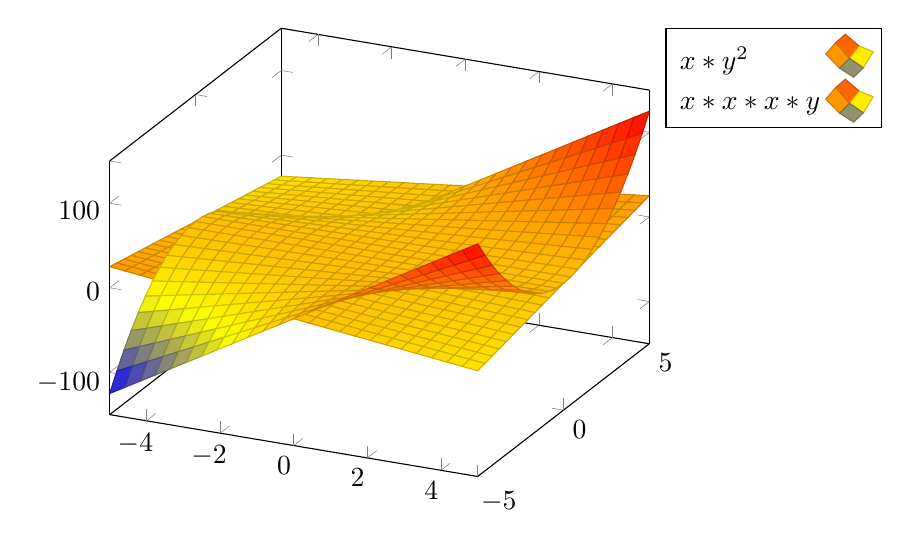
\begin{tikzpicture} 
\begin{axis}[
    % 图例的设置        
    legend style = {
    	% 设置图例锚点
    	anchor = north east,
        % 设置图例中 小图的对齐位置
    	cells = {anchor= east},
        },
    % 位置位置序号反转
    reverse legend,
    %设置图例水平显示的例数量   
    legend columns = 1,
    % 设置图例中图形的位置
    % legend plot pos=left|right|none
    legend plot pos= right,
    % 设置图例位置
    % legend pos=south west|south east|north west|north east|outer north east
    legend pos= outer north east,
    % 设置图例文字对齐方式
    % legend cell align=left|right|center
    legend cell align = left,
    % legend entries={
	   %  $x*x* x* y $,
	   %  $ x* y^2 $
	   %  },
    ]
\addplot3 [surf] {x*y};
\addlegendentry{$x*x* x* y $}
\addplot3 [surf] {x*y^2};
\addlegendentry{$ x* y^2 $}
\end{axis}
\end{tikzpicture}
\end{document}











